\documentclass{beamer}
\usetheme{ConnectivityLab}
\usepackage{times}
\usepackage{graphicx}
\usepackage{verbatim}
\usepackage{outlines}
\usepackage{fancyhdr}
\usepackage{subfigure}
\usepackage{cancel}
\usepackage{bibentry}
\usepackage{varwidth}
\usepackage{etoolbox}
\usepackage{epstopdf}

%%%%%%%%%%%%%%%%%%%%%%%%%%%%%%%%%%%%%%%%%%%%%%%%%%%%%%
%%%%%%%%%%%%%%%%%%%%%%%%%%%%%%%%%%%%%%%%%%%%%%%%%%%%%%

\title {
    Adaptive RACH Congestion Management to Support M2M Communication in 4G LTE Networks \cite{6802879}
}
\author {
    Yin-Hong, Hsu
}
\date {
    10 24, 2016
}

%%%%%%%%%%%%%%%%%%%%%%%%%%%%%%%%%%%%%%%%%%%%%%%%%%%%%%
%%%%%%%%%%%%%%%%%%%%%%%%%%%%%%%%%%%%%%%%%%%%%%%%%%%%%%

\begin{document}
\begin{frame}
    \titlepage
\end{frame}

%%%%%%%%%%%%%%%%%%%%%%%%%%%%%%%%%%%%%%%%%%%%%%%%%%%%%%
%%%%%%%%%%%%%%%%%%%%%%%%%%%%%%%%%%%%%%%%%%%%%%%%%%%%%%

\begin{frame}{Outline}
    \tableofcontentsgather
    \tableofcontents
\end{frame}

%%%%%%%%%%%%%%%%%%%%%%%%%%%%%%%%%%%%%%%%%%%%%%%%%%%%%%
%%%%%%%%%%%%%%%%%%%%%%%%%%%%%%%%%%%%%%%%%%%%%%%%%%%%%%
\section{Aim}

%%%%%%%%%%%%%%%%%%%%%%%%%%%%%%%%%%%%%%%%%%%%%%%%%%%%%%
%%%%%%%%%%%%%%%%%%%%%%%%%%%%%%%%%%%%%%%%%%%%%%%%%%%%%%
\begin{frame} {Aim} 
    \begin{itemize}
        \item \textbf{Proposed a adaptive RACH congestion management function (ARC)}
        \item \textbf{Adaptively chooses the most efficient congestion handling method to overcome from congestion}
    \end{itemize}
\end{frame}

%%%%%%%%%%%%%%%%%%%%%%%%%%%%%%%%%%%%%%%%%%%%%%%%%%%%%%
%%%%%%%%%%%%%%%%%%%%%%%%%%%%%%%%%%%%%%%%%%%%%%%%%%%%%%
\section{Background}

\begin{frame}{Background}
    \begin{figure}[t]
        \centering
        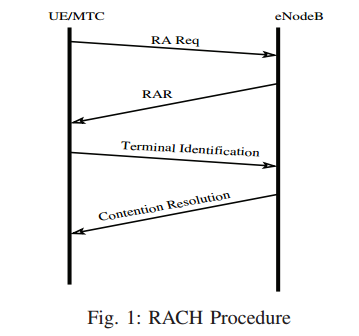
\includegraphics[width=0.7\textwidth]{figures/p1.png}
        \setbeamerfont{caption}{size=\tiny}
    \end{figure}
\end{frame}

%%%%%%%%%%%%%%%%%%%%%%%%%%%%%%%%%%%%%%%%%%%%%%%%%%%%%%
%%%%%%%%%%%%%%%%%%%%%%%%%%%%%%%%%%%%%%%%%%%%%%%%%%%%%%
\section{Proposed solution}
\begin{frame}{{Proposed solution}}
    \begin{itemize}
        \item{Various methods were discussed to handle the RACH congestion }
        \begin{itemize}    
            \item[-]{e.g. slotted access/ p-persistent/ numbering scheme...}
        \end{itemize}
        \item{Divide the RACH congestion level into three categories}
        \begin{itemize}    
            \item[-]{no congestion}
            \item[-]{moderate congestion}
            \item[-]{extreme congestion}
        \end{itemize}
    \end{itemize}
\end{frame}
\begin{frame}{{Proposed solution - algorithm}}
    \begin{itemize}
        \item{best congestion handling method selection algorithm (BCHMS)}
        \begin{itemize} 
            \item[-]{pick the best congestion handling method in specific congestion level}
        \end{itemize}
        \item{congestion estimation algorithm}
        \begin{itemize} 
            \item[-]{return the current congestion level}
        \end{itemize}
    \end{itemize}
\end{frame}
\begin{frame}{{Proposed solution - ARC algorithm}}
    \begin{itemize}
        \item{adaptive RACH congestion handling algorithm}
        \item{main function for this paper}
        \item{call congestion estimation algo to detect the level of congestion}
        \item{apply the corresponding congestion handling method}
    \end{itemize}
\end{frame}

\section{Result}
\begin{frame}{Result}
    \begin{figure}[t]
        \centering
        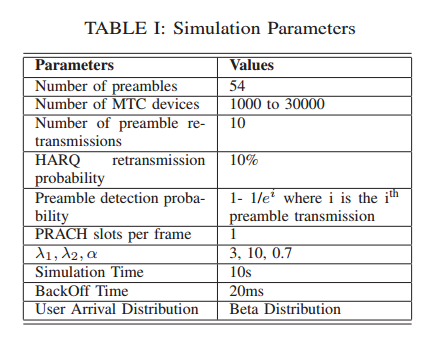
\includegraphics[width=0.8\textwidth]{figures/t1.png}
        \setbeamerfont{caption}{size=\tiny}
    \end{figure}
\end{frame}
\begin{frame}{Result}
    \begin{figure}[t]
        \centering
        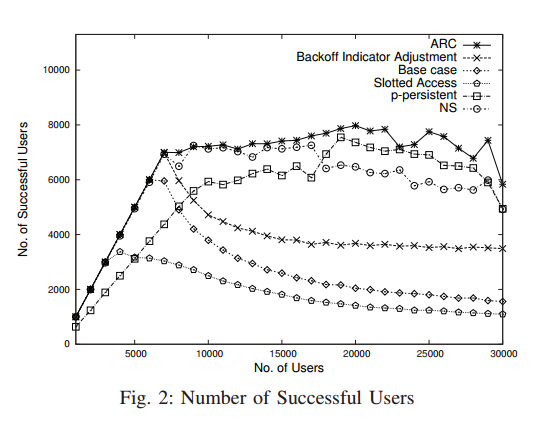
\includegraphics[width=0.8\textwidth]{figures/f1.png}
        \setbeamerfont{caption}{size=\tiny}
    \end{figure}
\end{frame}
\begin{frame}{Result}
    \begin{figure}[t]
        \centering
        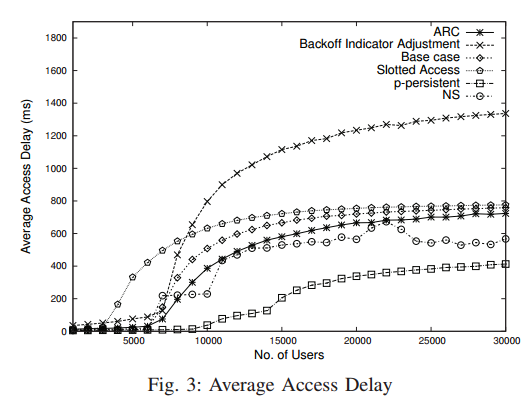
\includegraphics[width=0.8\textwidth]{figures/f2.png}
        \setbeamerfont{caption}{size=\tiny}
    \end{figure}
\end{frame}
\begin{frame}{Result}
    \begin{figure}[t]
        \centering
        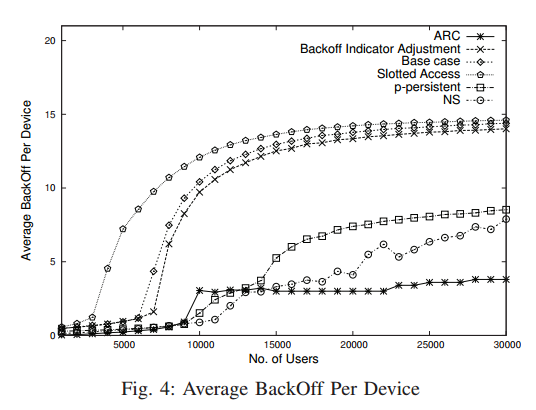
\includegraphics[width=0.8\textwidth]{figures/f3.png}
        \setbeamerfont{caption}{size=\tiny}
    \end{figure}
\end{frame}

%%%%%%%%%%%%%%%%%%%%%%%%%%%%%%%%%%%%%%%%%%%%%%%%%%%%%%
%%%%%%%%%%%%%%%%%%%%%%%%%%%%%%%%%%%%%%%%%%%%%%%%%%%%%%
\section{References}
\calcreferencespagetotal % Calc your References Page total number
\begin{frame}[allowframebreaks]{References}
    \fontsize{9pt}{13}\selectfont
    \bibliographystyle{IEEEtran}
    \bibliography{IEEEabrv,Citation}
\end{frame}

%%%%%%%%%%%%%%%%%%%%%%%%%%%%%%%%%%%%%%%%%%%%%%%%%%%%%%
%%%%%%%%%%%%%%%%%%%%%%%%%%%%%%%%%%%%%%%%%%%%%%%%%%%%%%
\section{}

\begin{frame}
    \centering
    \Large{Thanks for Your Attentions}
\end{frame}

\end{document}
